\section{Experiment on Request Reduction and Its Effect on Fault Detection} \label{sec:experiment}

The objective of the experiment is to examine whether the reduced
request set is as effective at fault detection as the original
request set. Similar to the goals of Hennessy et
al.~\cite{hennessy05:analysis} for grammar-based software, we wish
to investigate the following hypotheses:

%\begin{hypothesis}
We can achieve a significant reduction in request-set size for large
randomly generated request sets while maintaining equivalent policy,
rule, and condition coverage.
%\end{hypothesis}

%\begin{hypothesis}
Reducing a request set based on coverage will not proportionately
decrease its fault detection capability.
%\end{hypothesis}

\subsection{Metrics}

In order to investigate our hypotheses, we need to measure the
reduction in request-set size, the coverage metrics, and the
reduction in fault detection capability. The following metrics are
measured for each policy under test, each request set, and each
mutation operator.

\begin{itemize}

\item \emph{Policy hit percentage}. The policy hit percentage or
policy coverage is the number of applicable policies when evaluating
the request set divided by the total number of policies.

\item \emph{Rule hit percentage}. The rule hit percentage or rule
coverage is the number of applicable rules when evaluating the
request set divided by the total number of rules.

\item \emph{Condition hit percentage}. The condition hit percentage
is the number of hit true and hit false conditions when evaluating
the request set divided by two times of the total number of
conditions.

\item \emph{Test count}. The test count is the size of the request
set or the number of generated tests.  For testing access control
policies, a test is synonymous with request.

\item \emph{Reduced-test count}. Given a policy and the generated set
of requests, the reduced test count is the size of the reduced
request set based on policy coverage.

\item \emph{Mutant-killing ratio}. Given a request set, the policy
under test, and the set of generated mutants, the mutant-killing
ratio is the number of mutants killed by the request set divided by
the total number of mutants.

\end{itemize}

Intuitively a set of requests that achieve higher policy coverage
are more likely to reveal faults. This notion is easy to understand
because a fault in a policy element that is never covered by a
request would never contribute to a response and thus a fault in
that element cannot possibly be revealed. There is a direct
correlation between the test count and the test evaluation time.
Furthermore, a low test count is highly desirable because the
request-response pairs may need to be inspected manually to verify
that the policy specification exhibits the intended policy behavior.
An ideal request set should have a low test count, high structural
coverage, and high fault-detection capability.

\subsection{Results}

\begin{table}[t]%[htdp]
\centering \caption{\label{table:subjects} Policies used in the
experiment.}
\begin{small}
\begin{tabular}{|l|r|r|r|r|} \hline

   Subject &  \# PolSet &     \# Pol &    \# Rule &    \# Cond \\ \hline \hline

     codeA &          5 &          2 &          2 &          0 \\ \hline

     codeB &          7 &          3 &          3 &          0 \\ \hline

     codeC &          8 &          4 &          4 &          0 \\ \hline

     codeD &         11 &          5 &          5 &          0 \\ \hline

 default-2 &          1 &         13 &         13 &         12 \\ \hline

   demo-11 &          0 &          1 &          3 &          4 \\ \hline

   demo-26 &          0 &          1 &          2 &          2 \\ \hline

    demo-5 &          0 &          1 &          3 &          4 \\ \hline

mod-fedora &          1 &         13 &         13 &         12 \\
\hline

simple-policy &       1 &          2 &          2 &          0 \\
\hline

\end{tabular}
\end{small}
\end{table}

We used $10$ XACML policies collected from three different sources
as subjects in our experiment. Table~\ref{table:subjects} summarizes
the basic statistics of each policy. The first column shows the
subject names. Columns 2-5 show the numbers of policy sets,
policies, rules, and conditions, respectively. Five of the policies,
namely \CodeIn{simple-policy}, \CodeIn{codeA}, \CodeIn{codeB},
\CodeIn{codeC}, and \CodeIn{codeD} are examples used by Fisler et
al.~\cite{fisler05:verification,greenberg05:soundness}. The
remaining policies are examples of real XACML policies used by
Fedora\footnote{\url{http://www.fedora.info}}. Fedora is an open
source software that gives organizations a flexible service-oriented
architecture for managing and delivering digital content. Fedora
uses XACML to provide fine-grained access control to the digital
content that it manages. The Fedora repository of default and
example XACML policies provides a useful resource of realistic
subjects.

%%%%%%%%%%%%%%%%%%%%%%%%%%%%%%%%%%%%%%%%%%%%%%

We preprocessed each policy to ensure unique policy element
identifiers in order to correctly measure structural coverage. Once
each policy has been preprocessed, we randomly generate requests for
each policy as outlined in Section~\ref{sec:reqgen} (we configure
that 50 requests are randomly generated for each policy). As these
requests are generated and evaluated, we greedily select a smaller
set of requests with equivalent coverage as outlined in
Section~\ref{sec:reqreduce}.  If we define the size of the entire
request set as $r$ and the size of the reduced request set as $r'$
then we can define the reduction in request-set size,
$SizeReduction$, as follows:
\begin{displaymath}
SizeReduction = 1 - \frac{r'}{r}
\end{displaymath}

\begin{table*}[t]
    \centering
    \caption{Structural coverage, number of requests, and size reduction for each policy.}
    \label{table:coverage}
    \begin{small}
% Table generated by Excel2LaTeX from sheet 'icics'
\begin{tabular}{|r|r|r|r|r|r|r|}
\hline
   Subject &     Policy Hit &    Rule Hit &    Cond Hit &     \#Req &  \#Reduced Req &    Size Reduction \\
\hline \hline
     codeA &   100.00\% &   100.00\% &     - &         50 &          2 &       0.96 \\\hline

     codeB &   100.00\% &   100.00\% &     - &         50 &          3 &       0.94 \\\hline

     codeC &   100.00\% &   100.00\% &     - &         50 &          6 &       0.88 \\\hline

     codeD &   100.00\% &   100.00\% &     - &         50 &          6 &       0.88 \\\hline

 default-2 &   100.00\% &    92.31\% &    75.00\% &         50 &          6 &       0.88 \\\hline

   demo-11 &   100.00\% &   100.00\% &    75.00\% &         50 &          2 &       0.96 \\\hline

   demo-26 &   100.00\% &   100.00\% &    50.00\% &         50 &          1 &       0.98 \\\hline

    demo-5 &   100.00\% &   100.00\% &    75.00\% &         50 &          3 &       0.94 \\\hline

mod-fedora &   100.00\% &    84.62\% &    58.33\% &         50 &
7 &       0.86 \\\hline

simple-policy &   100.00\% &   100.00\% &     - &         50 &          4 &       0.92 \\
\hline
\end{tabular}
\end{small}
\end{table*}

Columns 2-7 of Table~\ref{table:coverage} show the three structural
coverage metrics, size of the generated request set, the size of the
reduced request set, and the computed size reduction for each
policy, respectively. A dash indicates that there are no policy
elements of that type and thus coverage cannot be computed. The
random request set achieves $100\%$ policy coverage for all subjects
because it is the most coarse measure of structural coverage. Rule
coverage and condition coverage are a finer measure of structural
coverage and thus more difficult to achieve with randomly generated
requests. The results show that we can achieve an average $92\%$
size reduction for the ten policies. The results suggest that we can
indeed greatly reduce the request set size of relatively large
randomly generated request sets while maintaining equivalent policy,
rule, and condition coverage.

\begin{figure}[t]
    \centering
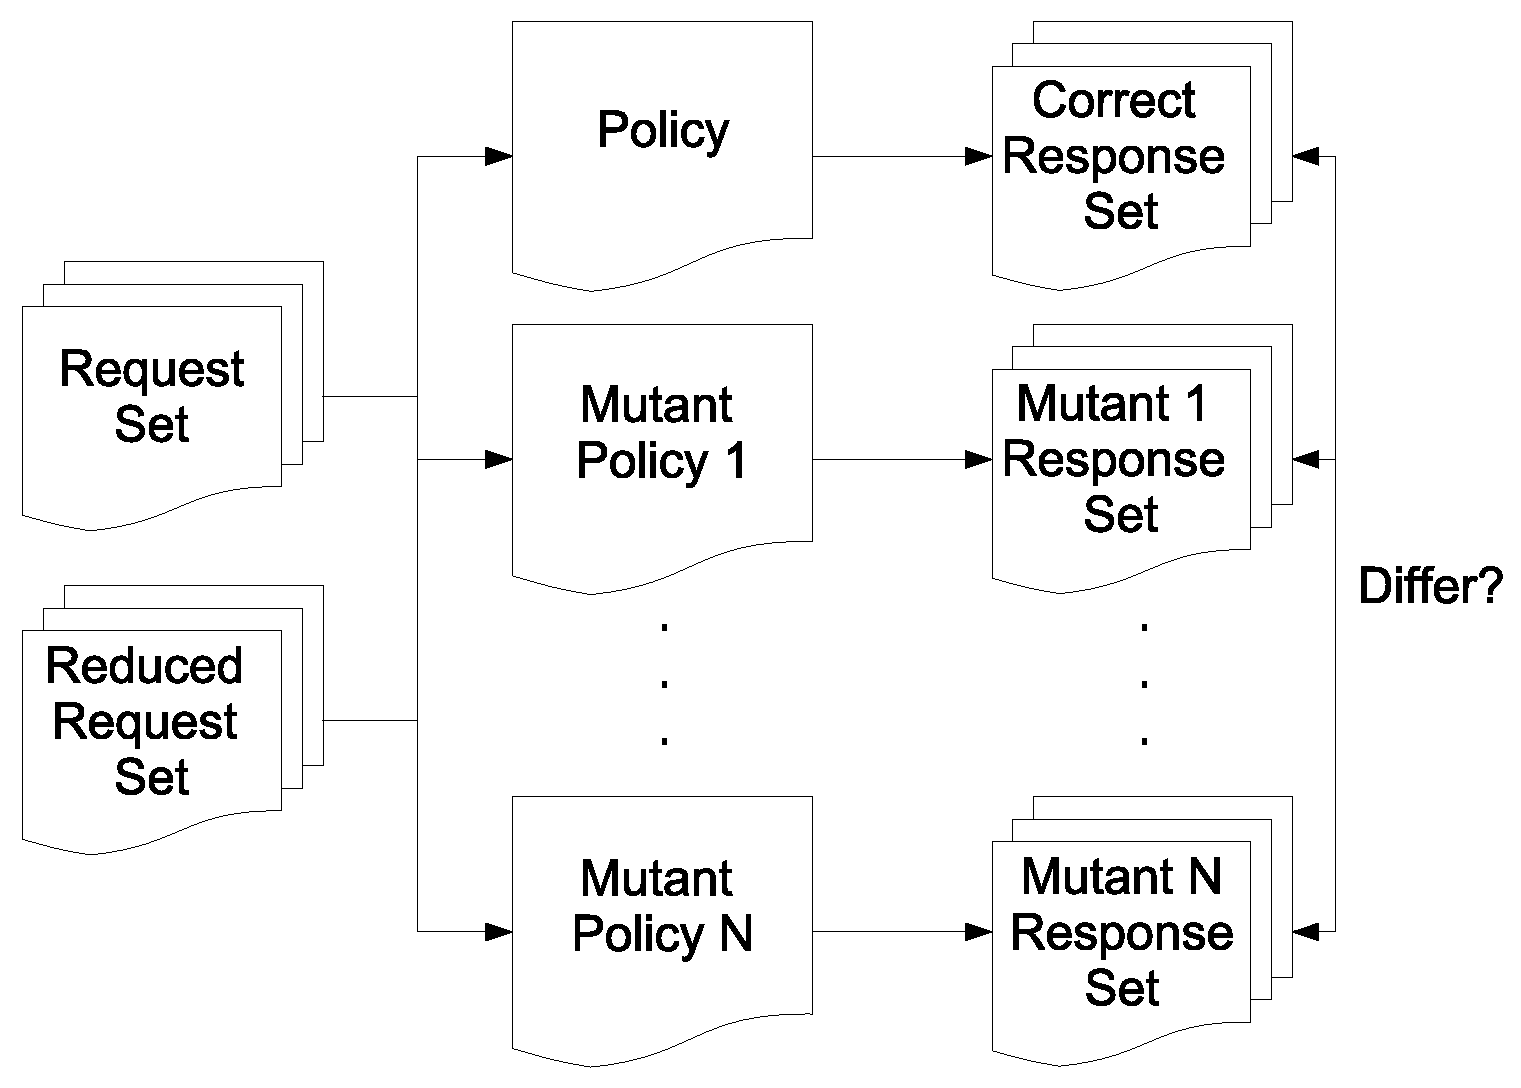
\includegraphics[width=3in]{coverage/mutant-exp}
\caption{Overview of fault detection experiment.}
\label{fig:mutant_exp}
\end{figure}

The second objective of the experiment is to investigate if the
reduced request set can still effectively detect faults in policies
compared to the full set. We perform the experiment illustrated in
Figure~\ref{fig:mutant_exp}.  The basic approach is to exploit
mutation testing as a mechanism to compare the fault-detection
capability of various request sets.  As discussed in
Section~\ref{sec:mutation}, we create several mutant policies using
the mutation operators listed in Table~\ref{table:mutationops} for
each of the experimental subjects. Each request set is executed
against each mutant policy and their corresponding responses are
recorded.  If the response for any request evaluated against the
original policy differs from the response for the request evaluated
against the mutant policy, then the mutant is said to be killed. We
define the $CapabilityReduction$ as a metric that quantifies the
relative fault detection capability of the reduced set compared to
its original set. If we define the total number of mutants detected
by the original set as $m$ and the total number of mutants detected
by the reduced set as $m'$, then we compute the reduction in fault
detection as:
\begin{displaymath}
CapabilityReduction=1 - \frac{m'}{m}
\end{displaymath}
\begin{figure}[t]
\centering
        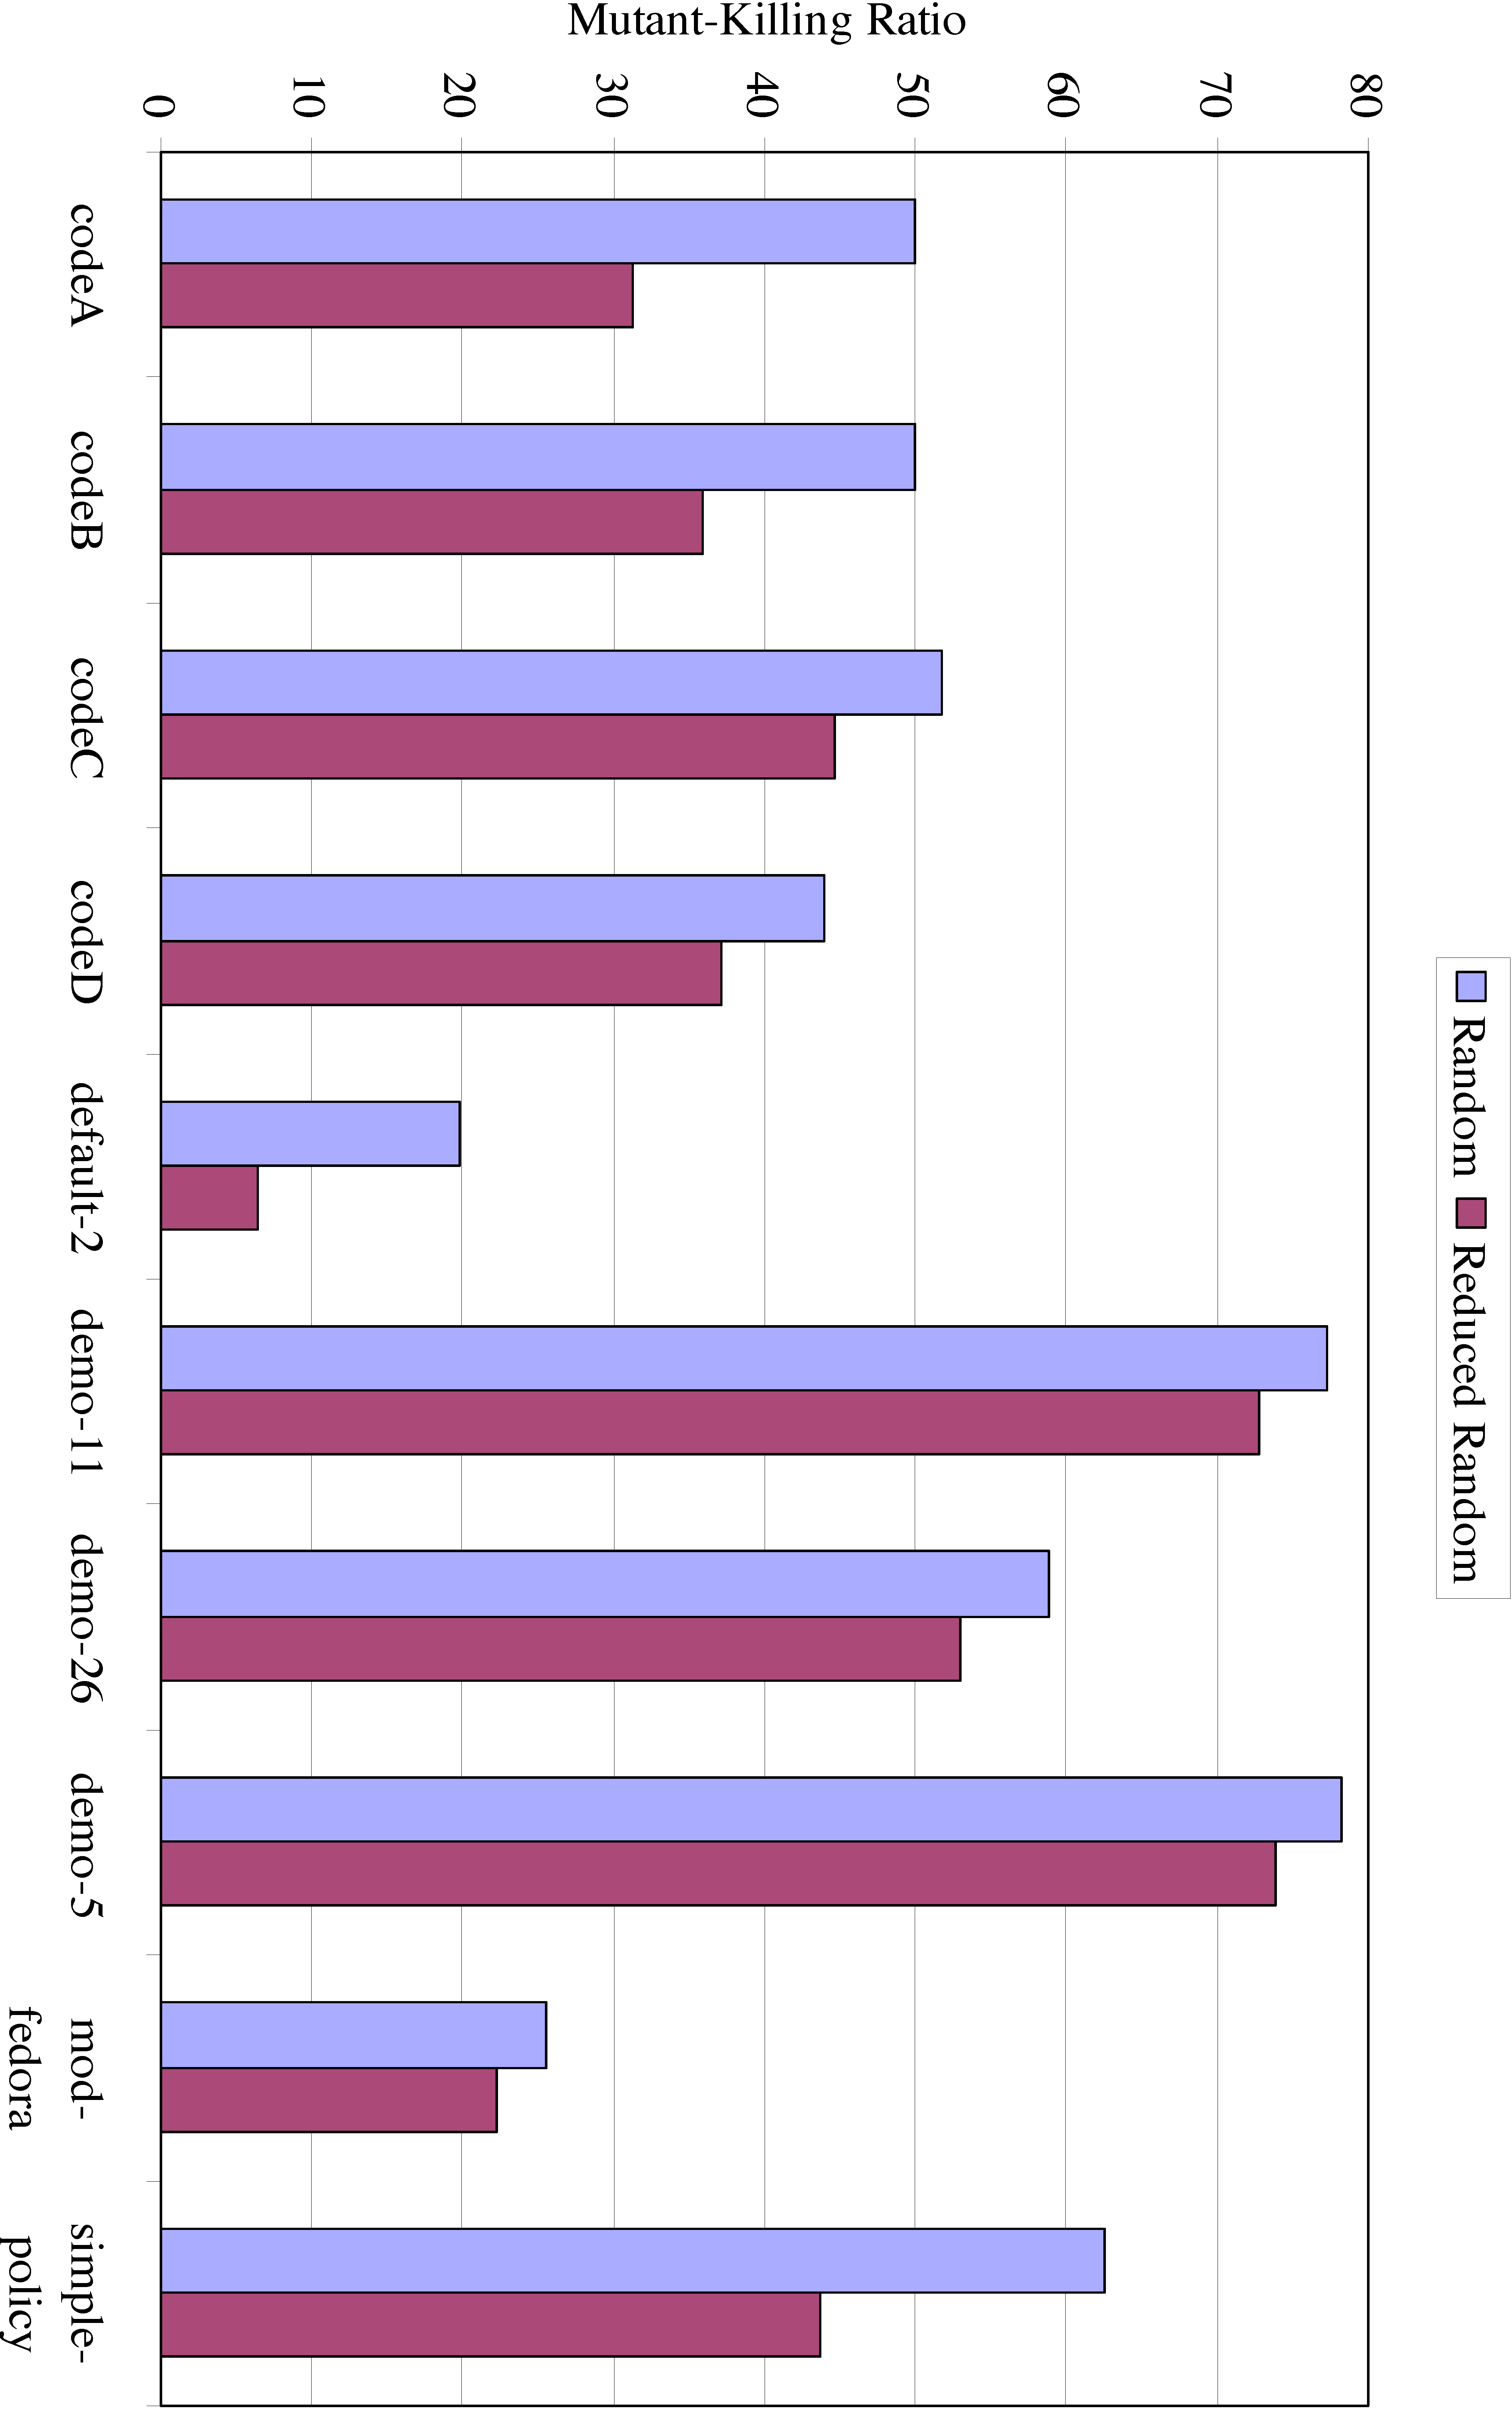
\includegraphics[width=3in]{coverage/kill-by-subj}
    \caption{\label{fig:killbysubj}Mutant-killing ratios for all operators by subjects.}
\end{figure}
Figure~\ref{fig:killbysubj} illustrates the average mutant-killing
ratios for each request set grouped by subjects. We observe that the
mutant-killing ratios across all subjects for the random and reduced
random request sets are quite similar. Unfortunately the
mutant-killing ratio is still low when considering the high
structural coverage. The observation indicates that a stronger
criteria is needed. Specifically the average mutant-killing ratios
for the Random, and Reduced Random request sets are $51.8\%$ and
$42.1\%$, respectively. Table~\ref{table:mutantkill} lists the
mutant-kill ratios in tabular format along with the computed
capability reduction. In summary, we observe a $92\%$ reduction in
size of the requests while only a $23\%$ reduction in fault
detection capability.

\begin{table}
\centering
    \caption{Mutant-killing ratios and capability reduction for each request set and each policy.}
    \label{table:mutantkill}
    \begin{small}
% Table generated by Excel2LaTeX from sheet 'icics'
\begin{tabular}{|l|r|r|r|}
\hline
   Subject &     Random & Reduced Random & Capability Reduction \\
\hline \hline
     codeA &    50.00\% &    31.25\% &    37.50\% \\
\hline
     codeB &    50.00\% &    35.87\% &    28.26\% \\
\hline
     codeC &    51.79\% &    44.64\% &    13.79\% \\
\hline
     codeD &    43.92\% &    37.16\% &    15.38\% \\
\hline
 default-2 &    19.75\% &     6.37\% &    67.74\% \\
\hline
   demo-11 &    77.27\% &    72.73\% &     5.88\% \\
\hline
   demo-26 &    58.82\% &    52.94\% &    10.00\% \\
\hline
    demo-5 &    78.26\% &    73.91\% &     5.56\% \\
\hline
mod-fedora &    25.48\% &    22.29\% &    12.50\% \\
\hline
simple-policy &    62.50\% &    43.75\% &    30.00\% \\
\hline
\end{tabular}
\end{small}
\end{table}

\Comment{Finally we provided the original policy and each mutant
policy to Margrave's change-impact analysis feature to perform
equivalent-mutant detection. If Margrave finds counter-examples that
illustrate differences between the policies, then they \emph{must
not} be equivalent. Unfortunately Margrave supports only a subset of
XACML features; therefore, the converse does not hold, resulting in
potential false positives. In other words, if Margrave does
\emph{not} find counter-examples for a particular mutant, then the
mutant \emph{may} or \emph{may not} be equivalent. In our
experiment, Margrave identified less than $1\%$ of all mutants as
potentially equivalent. Furthermore, these potentially equivalent
mutants occurred only for the CPC and CRC mutation operators.
Performing equivalent mutation detection is costly, taking
approximately $45$ minutes for the whole experiment. When
considering the low percentage of detection, potential for false
positives, and high computational cost, we feel other means of
equivalent mutant detection are needed.}

In summary, the results indicate that structural coverage is indeed
correlated to fault-detection capability. But structural coverage is
still not strong enough to achieve an acceptable level of fault
detection. Note that the structural coverage investigated in this
experiment is essentially equivalent to statement coverage in
general-purpose programming languages. In future work, we plan to
investigate stronger criteria that correspond to path coverage. We
expect these stronger criteria to be much more effective at
achieving higher killing ratios.\Comment{ Similar to the findings in
mutation testing of general-purpose programming languages, we found
that equivalent-mutant detection is expensive.}

\subsection{Threats to Validity}

The threats to external validity primarily include the degree to
which the subject policies, mutation operators, coverage metrics,
and test sets are representative of true practice. These threats
could be reduced by further experimentation on a wider type and
larger number of policies and an larger number of mutation
operators. In particular, lower level mutation operators are needed
to operate on the subject, resource, and action attributes found in
various policy elements. Currently the proposed mutation operators
operate only on higher level policy elements. The threats to
internal validity are instrumentation effects that can bias our
results such as faults in Sun's XACML implementation as well as
faults in our own policy mutator, policy coverage measurement tool,
and request generator.

%%%%%%%%%%%%%%%%%%%%%%%%%%%%%

\Comment{



The quantity and type of mutation operator used for each policy is
summarized in Table~\ref{table:mutants}.

\begin{table}[htdp]
\caption{\label{table:mutants}Type of mutation operator and
quantity of mutant policies created for each policy.}
\begin{center}
\begin{tabular}{|l|r|r|r|}
\hline Policy & apia-tighten & demo-5 & default \\
\hline
\hline Mutation Operator Id &&& \\
\hline REff & 2 & 3 & 13\\
\hline PTargT & 1 & 1 & 13\\
\hline PTargF & 1 & 1 & 13\\
\hline RTargT & 2 & 2 & 0\\
\hline RTargF & 2 & 2 & 0\\
\hline CondT & 2 & 2 & 6\\
\hline CondF & 2 & 2 & 6\\
\hline POrder & 0 & 0 & 0 \\
\hline ROrder & 1 & 5 & \\
\hline
\hline Total Mutants & 13 & 18 & 51 \\
\hline
\end{tabular}
\end{center}
\end{table}



Table~\ref{table:capreduce} summarizes the results of our
experiments on the reduction of fault detection.  The results
suggest that, on average, a 98.5\% reduction in request-set size
only results in a 18.97\% reduction in fault detection capability.
In many cases we suspect the reduction in fault detection
capability is acceptable considering the large reduction in
request-set size.  These results suggest that request sets
requiring manual inspection can be greatly reduced with relatively
low loss to fault detection capability.

\begin{table}[htdp]
\caption{\label{table:capreduce}Reduction in fault detection.}
\begin{center}
\begin{tabular}{|l|r|r|r|}
\hline Policy & apia-tighten & demo-5 & default \\
\hline \# Mutants & 13 & 18 & 51 \\
\hline Kill \% &&& \\
Original Set & 76.92\% & 94.44\% & 80.39\% \\
Reduced Set & 69.23\% & 77.78\% & 56.86\% \\
\hline Capability Reduction & 10\% & 17.65\% & 29.27\% \\
\hline
\end{tabular}
\end{center}
\end{table}

One possible explanation as to why the reduced set suffers from a
reduction in fault detection capability is greedy selection of
requests for addition to the reduced set.  Since requests can
carry multiple attribute values for the same attribute ids, it is
possible that two requests with the identical coverage can produce
different responses by operating on the same conditions in
different ways. There may be more optimal, albeit likely more
complex, algorithms for choosing requests.

We consider these results promising yet further experimentation with
larger, more complex policies and a more comprehensive suite of
mutation operators is necessary to further validate the findings.
We will investigate if there are any specific types of mutation
operators that result in mutants that are least likely to be killed
by the reduced set. }

%%%%%%%%%%%%%%%%%%%%%%%%%%%%%%%%%%%%%%%%%%%%%%%%%%%%%%%%%%
